\section{Circuitos combinacionais}

\frame{
	\frametitle{Relembrando...}
	
	\centering
	\begin{tikzpicture}[node distance=0.5cm, base/.style={
		% The shape:
		rectangle,minimum height=1cm,minimum width=1.5cm,rounded corners=3mm,align=center,
		% The rest
		very thick,draw=black!50,
		fill=black!20}]
	
	\node[base] (S) {Situação};
	\node[base,right=of S,text width=1.5cm] (TV) {Tabela verdade};
	\node[base, right=of TV, text width=2cm] (ES) {Expressão simplificada};
	\node[base, right=of ES] (C) {Circuito};
	
	\graph {(S) -> (TV) -> (ES) -> (C);};
	
	\end{tikzpicture}
%	\centerline{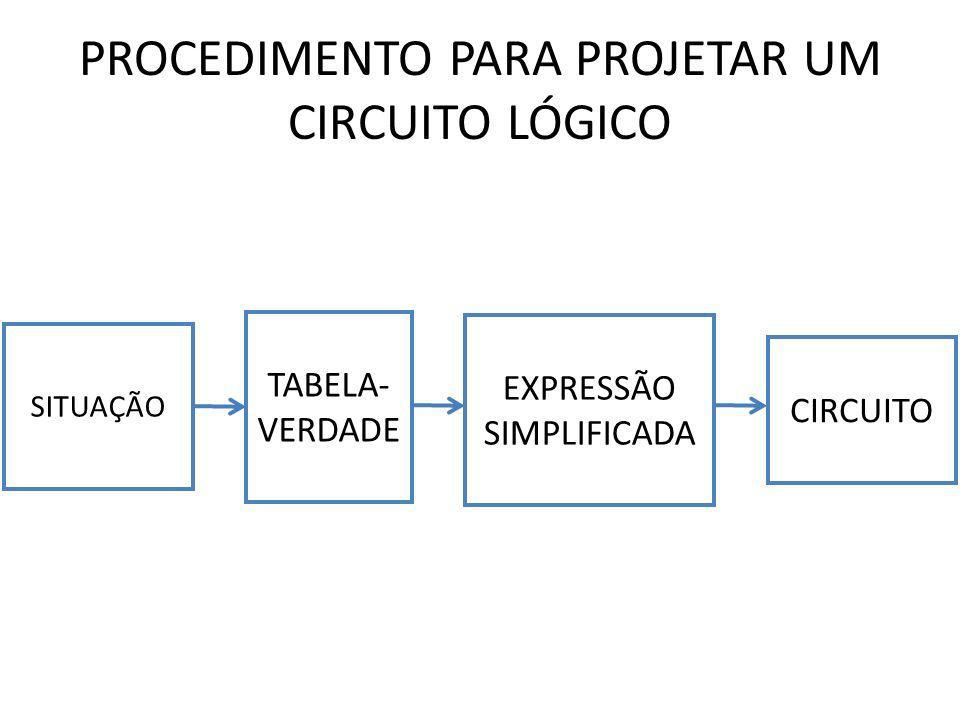
\includegraphics[width=0.75\linewidth]{Figuras/Ch4/resumo04.png}}
}

\frame{
	\frametitle{Circuitos combinacionais com 2 variáveis - Exemplo \#01}

	\centering
	

\tikzset{every picture/.style={line width=0.75pt}} %set default line width to 0.75pt        

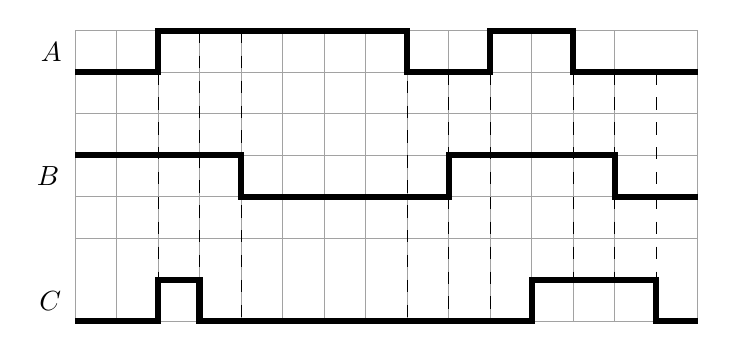
\begin{tikzpicture}[x=0.75pt,y=0.75pt,yscale=-1,xscale=1]
%uncomment if require: \path (0,300); %set diagram left start at 0, and has height of 300

%Shape: Grid [id:dp34531111101152123] 
\draw  [draw opacity=0] (100,40) -- (400,40) -- (400,180) -- (100,180) -- cycle ; \draw  [color={rgb, 255:red, 162; green, 162; blue, 162 }  ,draw opacity=1 ] (120,40) -- (120,180)(140,40) -- (140,180)(160,40) -- (160,180)(180,40) -- (180,180)(200,40) -- (200,180)(220,40) -- (220,180)(240,40) -- (240,180)(260,40) -- (260,180)(280,40) -- (280,180)(300,40) -- (300,180)(320,40) -- (320,180)(340,40) -- (340,180)(360,40) -- (360,180) ; \draw  [color={rgb, 255:red, 162; green, 162; blue, 162 }  ,draw opacity=1 ] (100,60) -- (400,60)(100,80) -- (400,80)(100,100) -- (400,100)(100,120) -- (400,120)(100,140) -- (400,140) ; \draw  [color={rgb, 255:red, 162; green, 162; blue, 162 }  ,draw opacity=1 ] (100,40) -- (400,40) -- (400,180) -- (100,180) -- cycle ;
%Straight Lines [id:da9908667716444586] 
\draw  [dash pattern={on 4.5pt off 4.5pt}]  (140,60) -- (140,160) ;


%Straight Lines [id:da9489034074703155] 
\draw  [dash pattern={on 4.5pt off 4.5pt}]  (160,40) -- (160,160) ;


%Straight Lines [id:da7444148673969375] 
\draw  [dash pattern={on 4.5pt off 4.5pt}]  (180,40) -- (180,180) ;


%Straight Lines [id:da33359589579811755] 
\draw  [dash pattern={on 4.5pt off 4.5pt}]  (260,40) -- (260,180) ;


%Straight Lines [id:da1689198722872045] 
\draw  [dash pattern={on 4.5pt off 4.5pt}]  (280,60) -- (280,180) ;


%Straight Lines [id:da2835936693187402] 
\draw  [dash pattern={on 4.5pt off 4.5pt}]  (300,60) -- (300,180) ;


%Straight Lines [id:da7069604701418795] 
\draw  [dash pattern={on 4.5pt off 4.5pt}]  (340,60) -- (340,160) ;


%Straight Lines [id:da35256438922338873] 
\draw  [dash pattern={on 4.5pt off 4.5pt}]  (360,60) -- (360,160) ;


%Straight Lines [id:da8396949759627998] 
\draw  [dash pattern={on 4.5pt off 4.5pt}]  (380,60) -- (380,160) ;


%Straight Lines [id:da8850959184881091] 
\draw [line width=2.25]    (100,60) -- (140,60) -- (140,40) -- (260,40) -- (260,60) -- (300,60) -- (300,40) -- (340,40) -- (340,60) -- (400,60) ;


%Straight Lines [id:da2574956876601695] 
\draw [line width=2.25]    (100,180) -- (140,180) -- (140,160) -- (160,160) -- (160,180) -- (320,180) -- (320,160) -- (380,160) -- (380,180) -- (400,180) ;


%Straight Lines [id:da8609754683162194] 
\draw [line width=2.25]    (100,100) -- (180,100) -- (180,120) -- (280,120) -- (280,100) -- (360,100) -- (360,120) -- (400,120) ;



% Text Node
\draw (88.5,50) node   {$A$};
% Text Node
\draw (87,110) node   {$B$};
% Text Node
\draw (88,170) node   {$C$};


\end{tikzpicture}

%	\centerline{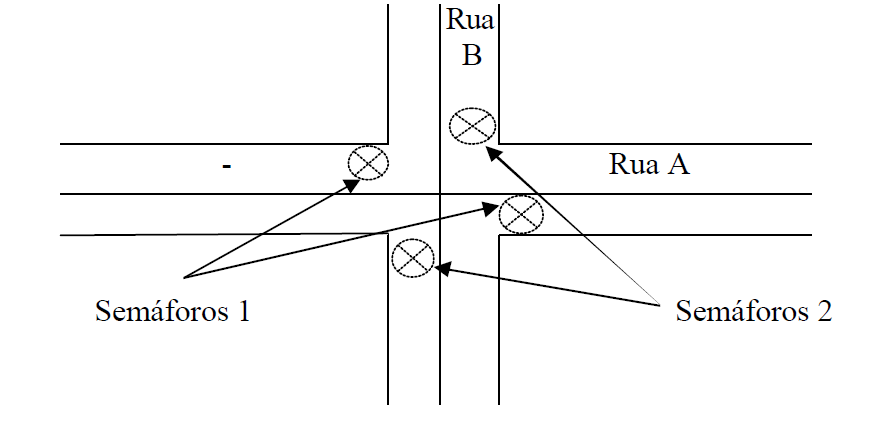
\includegraphics[width=0.75\linewidth]{Figuras/Ch4/2var.PNG}}
}

\frame{
	\frametitle{Circuitos combinacionais com 2 variáveis - Exemplo \#01}
	\begin{block}{}
		Deseja-se instalar, no cruzamento, um sistema automático de semáforos, com as seguintes características:
		\begin{itemize}
			\item Quando houver carros transitando somente na rua B, o semáforo 2 deverá permanecer verde para os carros trafegarem livremente.
			\item Igualmente, quando houver carros transitando somente na rua A, o semáforo 1 deverá permanecer verde.
			\item Quando houver carros transitando em ambas as ruas, o semáforo da rua A deve ficar verde, pois é a rua preferencial.
		\end{itemize}
	\end{block}

}


\frame{
	\frametitle{Circuitos combinacionais com 2 variáveis - Exemplo \#01}
		\centering
		\begin{tabular}{cc|cccc}
			\toprule
			A & B & G1 & R1 & G2 & R2 \\ \midrule
			0 & 0 &    &    &    &    \\
			0 & 1 &    &    &    &    \\
			1 & 0 &    &    &    &    \\
			1 & 1 &    &    &    &    \\ \bottomrule
		\end{tabular}
}

\frame{
	\frametitle{Circuitos combinacionais com 2 variáveis - Exemplo \#01}
		\centering
		\begin{tabular}{cc|cccc}
			\toprule
			A                & B                & G1 & R1 & G2 & R2 \\ \midrule
			\textcolor{red}0 & \textcolor{red}0 &    &    &    &    \\
			0                & 1                &    &    &    &    \\
			1                & 0                &    &    &    &    \\
			1                & 1                &    &    &    &    \\ \bottomrule
		\end{tabular}
}

\frame{
	\frametitle{Circuitos combinacionais com 2 variáveis - Exemplo \#01}
		\centering
		\begin{tabular}{cc|cccc}
			\toprule
			A                & B                & G1                 & R1                 & G2                 & R2                 \\ \midrule
			\textcolor{red}0 & \textcolor{red}0 & \textcolor{blue} X & \textcolor{blue} X & \textcolor{blue} X & \textcolor{blue} X \\
			0                & 1                &                    &                    &                    &                    \\
			1                & 0                &                    &                    &                    &                    \\
			1                & 1                &                    &                    &                    &                    \\ \bottomrule
		\end{tabular}
}

\frame{
	\frametitle{Circuitos combinacionais com 2 variáveis - Exemplo \#01}
		\centering
		\begin{tabular}{cc|cccc}
			\toprule
			A                & B                & G1 & R1 & G2 & R2 \\ \midrule
			0                & 0                & X  & X  & X  & X  \\ 
			\textcolor{red}0 & \textcolor{red}1 &    &    &    &    \\ 
			1                & 0                &    &    &    &    \\ 
			1                & 1                &    &    &    &    \\ \bottomrule
		\end{tabular}
}

\frame{
	\frametitle{Circuitos combinacionais com 2 variáveis - Exemplo \#01}
		\centering
		\begin{tabular}{cc|cccc}
			\toprule
			A                & B                & G1                & R1                & G2                & R2                \\ \midrule
			0                & 0                & X                 & X                 & X                 & X                 \\ 
			\textcolor{red}0 & \textcolor{red}1 & \textcolor{blue}0 & \textcolor{blue}1 & \textcolor{blue}1 & \textcolor{blue}0 \\ 
			1                & 0                &                   &                   &                   &                   \\ 
			1                & 1                &                   &                   &                   &                   \\ \bottomrule
		\end{tabular}
}

\frame{
	\frametitle{Circuitos combinacionais com 2 variáveis - Exemplo \#01}
		\centering
		\begin{tabular}{cc|cccc}
			\toprule
			A                & B                & G1 & R1 & G2 & R2 \\ \midrule
			0                & 0                & X  & X  & X  & X  \\ 
			0                & 1                & 0  & 1  & 1  & 0  \\ 
			\textcolor{red}1 & \textcolor{red}0 &    &    &    &    \\ 
			1                & 1                &    &    &    &    \\ \bottomrule
		\end{tabular}
}

\frame{
	\frametitle{Circuitos combinacionais com 2 variáveis - Exemplo \#01}
		\centering
		\begin{tabular}{cc|cccc}
			\toprule
			A                & B                & G1                & R1                & G2                & R2                \\ \midrule
			0                & 0                & X                 & X                 & X                 & X                 \\ 
			0                & 1                & 0                 & 1                 & 1                 & 0                 \\ 
			\textcolor{red}1 & \textcolor{red}0 & \textcolor{blue}1 & \textcolor{blue}0 & \textcolor{blue}0 & \textcolor{blue}1 \\ 
			1                & 1                &                   &                   &                   &                   \\ \bottomrule
		\end{tabular}
}

\frame{
	\frametitle{Circuitos combinacionais com 2 variáveis - Exemplo \#01}
		\centering
		\begin{tabular}{cc|cccc}
			\toprule
			A                & B                & G1 & R1 & G2 & R2 \\ \midrule
			0                & 0                & X  & X  & X  & X  \\ 
			0                & 1                & 0  & 1  & 1  & 0  \\ 
			1                & 0                & 1  & 0  & 0  & 1  \\ 
			\textcolor{red}1 & \textcolor{red}1 &    &    &    &    \\ \bottomrule
		\end{tabular}
}

\frame{
	\frametitle{Circuitos combinacionais com 2 variáveis - Exemplo \#01}
		\centering
		\begin{tabular}{cc|cccc}
			\toprule
			A                & B                & G1                & R1                & G2                & R2                \\ \midrule
			0                & 0                & X                 & X                 & X                 & X                 \\ 
			0                & 1                & 0                 & 1                 & 1                 & 0                 \\ 
			1                & 0                & 1                 & 0                 & 0                 & 1                 \\ 
			\textcolor{red}1 & \textcolor{red}1 & \textcolor{blue}1 & \textcolor{blue}0 & \textcolor{blue}0 & \textcolor{blue}1 \\ \bottomrule
		\end{tabular}
}

\frame{
	\frametitle{Circuitos combinacionais com 2 variáveis - Exemplo \#01}
		\centering
		\begin{tabular}{cc|cccc}
			\toprule
			A & B & G1 & R1 & G2 & R2            \\ \midrule
			0 & 0 & X  & X  & X  & X             \\ 
			0 & 1 & 0  & 1  & 1  & 0             \\ 
			1 & 0 & 1  & 0  & 0  & 1             \\ 
			1 & 1 & 1  & 0  & 0  & 1             \\ \bottomrule
		\end{tabular}
}

\frame{
\frametitle{Circuitos combinacionais com 2 variáveis - Exemplo \#01}

\begin{center}

\begin{karnaugh-map}[2][2][1][$A$][$B$]
\manualterms{X,1,0,1}
\implicant{1}{3}
\end{karnaugh-map}

\begin{block}{Expressão simplificada}
	\[ G1 = {\color{red} A} \]
\end{block}

\end{center}
}

\frame{
\frametitle{Circuitos combinacionais com 2 variáveis - Exemplo \#01}

\begin{center}

\begin{karnaugh-map}[2][2][1][$A$][$B$]
\manualterms{X,0,1,0}
\implicant{0}{2}
\end{karnaugh-map}

\begin{block}{Expressão simplificada}
	\[ R1 = {\color{red} \notted{A}} \]
\end{block}

\end{center}
}

\frame{
\frametitle{Circuitos combinacionais com 2 variáveis - Exemplo \#01}

\begin{center}

\begin{karnaugh-map}[2][2][1][$A$][$B$]
\manualterms{X,0,1,0}
\implicant{0}{2}
\end{karnaugh-map}

\begin{block}{Expressão simplificada}
	\[ G2 = {\color{red} \notted{A}} \]
\end{block}

\end{center}
}

\frame{
\frametitle{Circuitos combinacionais com 2 variáveis - Exemplo \#01}

\begin{center}

\begin{karnaugh-map}[2][2][1][$A$][$B$]
\manualterms{X,1,0,1}
\implicant{1}{3}
\end{karnaugh-map}

\begin{block}{Expressão simplificada}
	\[ R2 = {\color{red} A} \]
\end{block}

\end{center}
}

\frame{
	\frametitle{Circuitos combinacionais com 3 variáveis - Exemplo \#02}
	\centerline{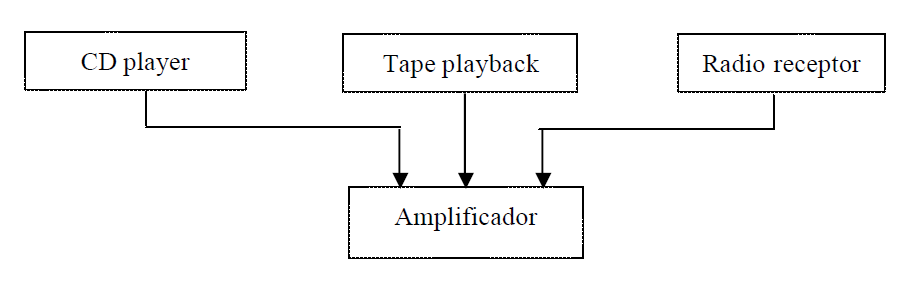
\includegraphics[width=1\linewidth]{Figuras/Ch4/3var.PNG}}
}

\frame{
	\frametitle{Circuitos combinacionais com 3 variáveis - Exemplo \#02}

	\begin{block}{}
		Deseja-se instalar um amplificador para ligar três aparelhos, com as seguintes prioridades: 
		
		\begin{itemize}
			\item Prioridade 1: CD player
			\item Prioridade 2: Tape playback
			\item Prioridade 3: Rádio receptor
		\end{itemize}
	\end{block}
}

\frame{
	\frametitle{Circuitos combinacionais com 3 variáveis - Exemplo \#02}
		\centering
		\begin{tabular}{ccc|ccc}
			\toprule
			A & B & C & SA & SB & SC             \\ \midrule
			0 & 0 & 0 &    &    &                \\ 
			0 & 0 & 1 &    &    &                \\ 
			0 & 1 & 0 &    &    &                \\ 
			0 & 1 & 1 &    &    &                \\ 
			1 & 0 & 0 &    &    &                \\ 
			1 & 0 & 1 &    &    &                \\ 
			1 & 1 & 0 &    &    &                \\ 
			1 & 1 & 1 &    &    &                \\ \bottomrule
		\end{tabular}
}

\frame{
	\frametitle{Circuitos combinacionais com 3 variáveis - Exemplo \#02}
		\centering
		\begin{tabular}{ccc|ccc}
			\toprule
			A                & B & C & SA & SB & SC \\ \midrule
			\textcolor{red}0 &
			\textcolor{red}0 &
			\textcolor{red}0 &   &   &              \\ 
			0                & 0 & 1 &    &    &    \\ 
			0                & 1 & 0 &    &    &    \\ 
			0                & 1 & 1 &    &    &    \\ 
			1                & 0 & 0 &    &    &    \\ 
			1                & 0 & 1 &    &    &    \\ 
			1                & 1 & 0 &    &    &    \\ 
			1                & 1 & 1 &    &    &    \\ \bottomrule
		\end{tabular}
}

\frame{
	\frametitle{Circuitos combinacionais com 3 variáveis - Exemplo \#02}
		\centering
		\begin{tabular}{ccc|ccc}
			\toprule
			A                & B                 & C                 & SA                & SB & SC \\ \midrule
			\textcolor{red}0 &
			\textcolor{red}0 &
			\textcolor{red}0 & \textcolor{blue}X & \textcolor{blue}X & \textcolor{blue}X           \\ 
			0                & 0                 & 1                 &                   &    &    \\ 
			0                & 1                 & 0                 &                   &    &    \\ 
			0                & 1                 & 1                 &                   &    &    \\ 
			1                & 0                 & 0                 &                   &    &    \\ 
			1                & 0                 & 1                 &                   &    &    \\ 
			1                & 1                 & 0                 &                   &    &    \\ 
			1                & 1                 & 1                 &                   &    &    \\ \bottomrule
		\end{tabular}
}


\frame{
	\frametitle{Circuitos combinacionais com 3 variáveis - Exemplo \#02}
		\centering
		\begin{tabular}{ccc|ccc}\toprule
			A                & B                & C                & SA & SB & SC \\ \midrule
			0                & 0                & 0                & X  & X  & X  \\ 
			\textcolor{red}0 & \textcolor{red}0 & \textcolor{red}1 &    &    &    \\ 
			0                & 1                & 0                &    &    &    \\ 
			0                & 1                & 1                &    &    &    \\ 
			1                & 0                & 0                &    &    &    \\ 
			1                & 0                & 1                &    &    &    \\ 
			1                & 1                & 0                &    &    &    \\ 
			1                & 1                & 1                &    &    &    \\ \bottomrule
		\end{tabular}
}

\frame{
	\frametitle{Circuitos combinacionais com 3 variáveis - Exemplo \#02}
		\centering
		\begin{tabular}{ccc|ccc}
			\toprule
			A                & B                & C                & SA                & SB                & SC                \\ \midrule
			0                & 0                & 0                & X                 & X                 & X                 \\ 
			\textcolor{red}0 & \textcolor{red}0 & \textcolor{red}1 & \textcolor{blue}0 & \textcolor{blue}0 & \textcolor{blue}1 \\ 
			0                & 1                & 0                &                   &                   &                   \\ 
			0                & 1                & 1                &                   &                   &                   \\ 
			1                & 0                & 0                &                   &                   &                   \\ 
			1                & 0                & 1                &                   &                   &                   \\ 
			1                & 1                & 0                &                   &                   &                   \\ 
			1                & 1                & 1                &                   &                   &                   \\ \bottomrule
		\end{tabular}
}

\frame{
	\frametitle{Circuitos combinacionais com 3 variáveis - Exemplo \#02}
		\centering
		\begin{tabular}{ccc|ccc}
			\toprule
			A                & B                & C                & SA & SB & SC \\ \midrule
			0                & 0                & 0                & X  & X  & X  \\ 
			0                & 0                & 1                & 0  & 0  & 1  \\ 
			\textcolor{red}0 & \textcolor{red}1 & \textcolor{red}0 &    &    &    \\ 
			0                & 1                & 1                &    &    &    \\ 
			1                & 0                & 0                &    &    &    \\ 
			1                & 0                & 1                &    &    &    \\ 
			1                & 1                & 0                &    &    &    \\ 
			1                & 1                & 1                &    &    &    \\ \bottomrule
		\end{tabular}
}

\frame{
	\frametitle{Circuitos combinacionais com 3 variáveis - Exemplo \#02}
		\centering
		\begin{tabular}{ccc|ccc}
			\toprule
			A                & B                & C                & SA                & SB                & SC                \\ \midrule
			0                & 0                & 0                & X                 & X                 & X                 \\ 
			0                & 0                & 1                & 0                 & 0                 & 1                 \\ 
			\textcolor{red}0 & \textcolor{red}1 & \textcolor{red}0 & \textcolor{blue}0 & \textcolor{blue}1 & \textcolor{blue}0 \\ 
			0                & 1                & 1                &                   &                   &                   \\ 
			1                & 0                & 0                &                   &                   &                   \\ 
			1                & 0                & 1                &                   &                   &                   \\ 
			1                & 1                & 0                &                   &                   &                   \\ 
			1                & 1                & 1                &                   &                   &                   \\ \bottomrule
		\end{tabular}
}

\frame{
	\frametitle{Circuitos combinacionais com 3 variáveis - Exemplo \#02}
		\centering
		\begin{tabular}{ccc|ccc}
			\toprule
			A                & B                & C                & SA & SB & SC \\ \midrule
			0                & 0                & 0                & X  & X  & X  \\ 
			0                & 0                & 1                & 0  & 0  & 1  \\ 
			0                & 1                & 0                & 0  & 1  & 0  \\ 
			\textcolor{red}0 & \textcolor{red}1 & \textcolor{red}1 &    &    &    \\ 
			1                & 0                & 0                &    &    &    \\ 
			1                & 0                & 1                &    &    &    \\ 
			1                & 1                & 0                &    &    &    \\ 
			1                & 1                & 1                &    &    &    \\ \bottomrule
		\end{tabular}
}

\frame{
	\frametitle{Circuitos combinacionais com 3 variáveis - Exemplo \#02}
		\centering
		\begin{tabular}{ccc|ccc}
			\toprule
			A                & B                & C                & SA                & SB                & SC                \\ \midrule
			0                & 0                & 0                & X                 & X                 & X                 \\ 
			0                & 0                & 1                & 0                 & 0                 & 1                 \\ 
			0                & 1                & 0                & 0                 & 1                 & 0                 \\ 
			\textcolor{red}0 & \textcolor{red}1 & \textcolor{red}1 & \textcolor{blue}0 & \textcolor{blue}1 & \textcolor{blue}0 \\ 
			1                & 0                & 0                &                   &                   &                   \\ 
			1                & 0                & 1                &                   &                   &                   \\ 
			1                & 1                & 0                &                   &                   &                   \\ 
			1                & 1                & 1                &                   &                   &                   \\ \bottomrule
		\end{tabular}
}


\frame{
	\frametitle{Circuitos combinacionais com 3 variáveis - Exemplo \#02}
		\centering
		\begin{tabular}{ccc|ccc}
			\toprule
			A                & B                & C                & SA & SB & SC \\ \midrule
			0                & 0                & 0                & X  & X  & X  \\ 
			0                & 0                & 1                & 0  & 0  & 1  \\ 
			0                & 1                & 0                & 0  & 1  & 0  \\ 
			0                & 1                & 1                & 0  & 1  & 0  \\ 
			\textcolor{red}1 & \textcolor{red}0 & \textcolor{red}0 &    &    &    \\ 
			1                & 0                & 1                &    &    &    \\ 
			1                & 1                & 0                &    &    &    \\ 
			1                & 1                & 1                &    &    &    \\ \bottomrule
		\end{tabular}
}

\frame{
	\frametitle{Circuitos combinacionais com 3 variáveis - Exemplo \#02}
		\centering
		\begin{tabular}{ccc|ccc}
			\toprule
			A                & B                & C                & SA                & SB                & SC                \\ \midrule
			0                & 0                & 0                & X                 & X                 & X                 \\ 
			0                & 0                & 1                & 0                 & 0                 & 1                 \\ 
			0                & 1                & 0                & 0                 & 1                 & 0                 \\ 
			0                & 1                & 1                & 0                 & 1                 & 0                 \\ 
			\textcolor{red}1 & \textcolor{red}0 & \textcolor{red}0 & \textcolor{blue}1 & \textcolor{blue}0 & \textcolor{blue}0 \\ 
			1                & 0                & 1                &                   &                   &                   \\ 
			1                & 1                & 0                &                   &                   &                   \\ 
			1                & 1                & 1                &                   &                   &                   \\ \bottomrule
		\end{tabular}
}

\frame{
	\frametitle{Circuitos combinacionais com 3 variáveis - Exemplo \#02}
		\centering
		\begin{tabular}{ccc|ccc}
			\toprule
			A                & B                & C                & SA & SB & SC \\ \midrule
			0                & 0                & 0                & X  & X  & X  \\ 
			0                & 0                & 1                & 0  & 0  & 1  \\ 
			0                & 1                & 0                & 0  & 1  & 0  \\ 
			0                & 1                & 1                & 0  & 1  & 0  \\ 
			1                & 0                & 0                & 1  & 0  & 0  \\ 
			\textcolor{red}1 & \textcolor{red}0 & \textcolor{red}1 &    &    &    \\ 
			1                & 1                & 0                &    &    &    \\ 
			1                & 1                & 1                &    &    &    \\ \bottomrule
		\end{tabular}
}

\frame{
	\frametitle{Circuitos combinacionais com 3 variáveis - Exemplo \#02}
		\centering
		\begin{tabular}{ccc|ccc}
			\toprule
			A                & B                & C                & SA                & SB                & SC                \\ \midrule
			0                & 0                & 0                & X                 & X                 & X                 \\ 
			0                & 0                & 1                & 0                 & 0                 & 1                 \\ 
			0                & 1                & 0                & 0                 & 1                 & 0                 \\ 
			0                & 1                & 1                & 0                 & 1                 & 0                 \\ 
			1                & 0                & 0                & 1                 & 0                 & 0                 \\ 
			\textcolor{red}1 & \textcolor{red}0 & \textcolor{red}1 & \textcolor{blue}1 & \textcolor{blue}0 & \textcolor{blue}0 \\ 
			1                & 1                & 0                &                   &                   &                   \\ 
			1                & 1                & 1                &                   &                   &                   \\ \bottomrule
		\end{tabular}
}

\frame{
	\frametitle{Circuitos combinacionais com 3 variáveis - Exemplo \#02}
		\centering
		\begin{tabular}{ccc|ccc}
			\toprule
			A                & B                & C                & SA & SB & SC \\ \midrule
			0                & 0                & 0                & X  & X  & X  \\ 
			0                & 0                & 1                & 0  & 0  & 1  \\ 
			0                & 1                & 0                & 0  & 1  & 0  \\ 
			0                & 1                & 1                & 0  & 1  & 0  \\ 
			1                & 0                & 0                & 1  & 0  & 0  \\ 
			1                & 0                & 1                & 1  & 0  & 0  \\ 
			\textcolor{red}1 & \textcolor{red}1 & \textcolor{red}0 &    &    &    \\ 
			1                & 1                & 1                &    &    &    \\ \bottomrule
		\end{tabular}
}

\frame{
	\frametitle{Circuitos combinacionais com 3 variáveis - Exemplo \#02}
		\centering
		\begin{tabular}{ccc|ccc}
			\toprule
			A                & B                & C                & SA                & SB                & SC                \\ \midrule
			0                & 0                & 0                & X                 & X                 & X                 \\ 
			0                & 0                & 1                & 0                 & 0                 & 1                 \\ 
			0                & 1                & 0                & 0                 & 1                 & 0                 \\ 
			0                & 1                & 1                & 0                 & 1                 & 0                 \\ 
			1                & 0                & 0                & 1                 & 0                 & 0                 \\ 
			1                & 0                & 1                & 1                 & 0                 & 0                 \\ 
			\textcolor{red}1 & \textcolor{red}1 & \textcolor{red}0 & \textcolor{blue}1 & \textcolor{blue}0 & \textcolor{blue}0 \\ 
			1                & 1                & 1                &                   &                   &                   \\ \bottomrule
		\end{tabular}
}

\frame{
	\frametitle{Circuitos combinacionais com 3 variáveis - Exemplo \#02}
		\centering
		\begin{tabular}{ccc|ccc}
			\toprule
			A                & B                & C                & SA & SB & SC \\ \midrule
			0                & 0                & 0                & X  & X  & X  \\ 
			0                & 0                & 1                & 0  & 0  & 1  \\ 
			0                & 1                & 0                & 0  & 1  & 0  \\ 
			0                & 1                & 1                & 0  & 1  & 0  \\ 
			1                & 0                & 0                & 1  & 0  & 0  \\ 
			1                & 0                & 1                & 1  & 0  & 0  \\ 
			1                & 1                & 0                & 1  & 0  & 0  \\ 
			\textcolor{red}1 & \textcolor{red}1 & \textcolor{red}1 &    &    &    \\ \bottomrule
		\end{tabular}
}

\frame{
	\frametitle{Circuitos combinacionais com 3 variáveis - Exemplo \#02}
		\centering
		\begin{tabular}{ccc|ccc}
			\toprule
			A                & B                & C                & SA                & SB                & SC                \\ \midrule
			0                & 0                & 0                & X                 & X                 & X                 \\ 
			0                & 0                & 1                & 0                 & 0                 & 1                 \\ 
			0                & 1                & 0                & 0                 & 1                 & 0                 \\ 
			0                & 1                & 1                & 0                 & 1                 & 0                 \\ 
			1                & 0                & 0                & 1                 & 0                 & 0                 \\ 
			1                & 0                & 1                & 1                 & 0                 & 0                 \\ 
			1                & 1                & 0                & 1                 & 0                 & 0                 \\ 
			\textcolor{red}1 & \textcolor{red}1 & \textcolor{red}1 & \textcolor{blue}1 & \textcolor{blue}0 & \textcolor{blue}0 \\ \bottomrule
		\end{tabular}
}

\frame{
	\frametitle{Circuitos combinacionais com 3 variáveis - Exemplo \#02}
		\centering
		\begin{tabular}{ccc|ccc}
			\toprule
			A & B & C & SA & SB & SC             \\ \midrule
			0 & 0 & 0 & X  & X  & X              \\ 
			0 & 0 & 1 & 0  & 0  & 1              \\ 
			0 & 1 & 0 & 0  & 1  & 0              \\ 
			0 & 1 & 1 & 0  & 1  & 0              \\ 
			1 & 0 & 0 & 1  & 0  & 0              \\ 
			1 & 0 & 1 & 1  & 0  & 0              \\ 
			1 & 1 & 0 & 1  & 0  & 0              \\ 
			1 & 1 & 1 & 1  & 0  & 0              \\ \bottomrule
		\end{tabular}
}

\frame{
\frametitle{Circuitos combinacionais com 3 variáveis - Exemplo \#02}

\begin{center}

\begin{karnaugh-map}[4][2][1][$AB$][$C$]
\manualterms{X,0,1,1,0,0,1,1}
\implicant{3}{6}
\end{karnaugh-map}

\begin{block}{Expressão simplificada}
	\[ SA = {\color{red} A} \]
\end{block}

\end{center}
}

\frame{
\frametitle{Circuitos combinacionais com 3 variáveis - Exemplo \#02}

\begin{center}

\begin{karnaugh-map}[4][2][1][$AB$][$C$]
\manualterms{X,1,0,0,0,1,0,0}
\implicant{1}{5}
\end{karnaugh-map}

\begin{block}{Expressão simplificada}
	\[ SB = {\color{red} \notted{A}\cdot B} \]
\end{block}

\end{center}
}

\frame{
\frametitle{Circuitos combinacionais com 3 variáveis - Exemplo \#02}

\begin{center}

\begin{karnaugh-map}[4][2][1][$AB$][$C$]
\manualterms{X,0,0,0,1,0,0,0}
\implicant{0}{4}
\end{karnaugh-map}

\begin{block}{Expressão simplificada}
	\[ SC = {\color{red} \notted{A}\cdot \notted{B}} \]
\end{block}

\end{center}
}


\section*{Exercícios}

\frame{
	\frametitle{Exercícios}
	\begin{block}{}
		01. Quatro juízes participam de um programa de calouros e cada um tem a sua disposição, uma chave liga/desliga correspondendo ao julgamento do candidato: aprovado ou reprovado. Na saída existem três lâmpadas, correspondentes a três resultados: aprovado (pela maioria), reprovado (pela maioria) ou empate.
		
		\bigskip
		
		02. Um motor deve funcionar quando uma ou mais das seguintes condições forem satisfeitas: \textbf{(1)} Regime de carga $\geqslant 80\%$ e Temperatura $> \SI{25}{\degreeCelsius}$; \textbf{(2)} Regime de carga $< 80\%$, Umidade relativa $>60\%$ e Temperatura $> \SI{25}{\degreeCelsius}$; \textbf{(3)} Regime de carga $< 80\%$, no período de carga entre as \SI{15}{\hour} e \SI{16}{\hour}; \textbf{(4)} Temperatura $> \SI{25}{\degreeCelsius}$, fora do período de carga entre as \SI{15}{\hour} e \SI{16}{\hour}.
		
		\bigskip
		
		03. Projete um circuito digital com 4 variáveis de entrada, que indique quando há um número primo	presente na entrada.
	\end{block}
}


\section*{Referências}


\frame{
	\frametitle{Referências e exercícios complementares}
	\begin{itemize}
		\item IDOETA, Ivan V. e CAPUANO, Francisco G. Elementos de Eletrônica Digital. São Paulo:
		      Editora Érica, ed. 40. 2008.
	\end{itemize}

	\centering{\alert{Página 174 - \textbf{4.3.1 até 4.3.8}}}

}